

\chapter{Réalisation et tests}
\section{Introduction}
Après avoir exposé en détail notre méthode automatique d'élagage dans le chapitre précèdent, nous discuterons maintenant sur les technologies et outils qui ont été choisis pour matérialiser cette approche et garantir son déploiement efficace. De ce fait, il est essentiel d'examiner en détail les langages de programmation, les bibliothèques et les frameworks qui ont été sélectionnés pour concrétiser notre approche. Nous offrons également un aperçu des stratégies de test que nous avons employées pour évaluer la performance de notre solution. Ces tests ont été établis pour mesurer les performances des modèles VGG-19 et ResNet-34 et la précision de chacun.

\section{Modèles et jeu de données utilisés}
Notre méthode d'élagage a été conçue pour élaguer les réseaux de neurones comportant seulement deux types de couches: les couches de convolution et les couches entièrement connectées. C'est pourquoi nous avons choisi d'utiliser des modèles tels que VGG-19 et ResNet-34. Dans cette section, nous parlerons de l'architecture et de l'organisation de ces deux modèles ainsi que le jeu de données CIFAR-10 qui est utilisé pour les entraîner.
\subsection{CIFAR-10}
CIFAR-10 \footnote{acronyme qui représente le "Canadian Institute for Advanced Research" (Institut canadien de recherches avancées)} est un jeu de données qui est souvent utilisé dans le domaine de la vision par ordinateur. Il se compose d'un total de 60 000 images en couleur de 32x32 pixels chacune, réparties en 10 classes différentes, avec 6 000 images par classe [\cite{krizhevsky2009learning}]. Ces 10 classes d'images comprennent: des avions, des automobiles, des oiseaux, des chats, des cerfs, des chiens, des grenouilles, des chevaux, des bateaux et des camions (\ref{fig:cifar-10-classes}).

\begin{figure}[hbt!]
  \centering
  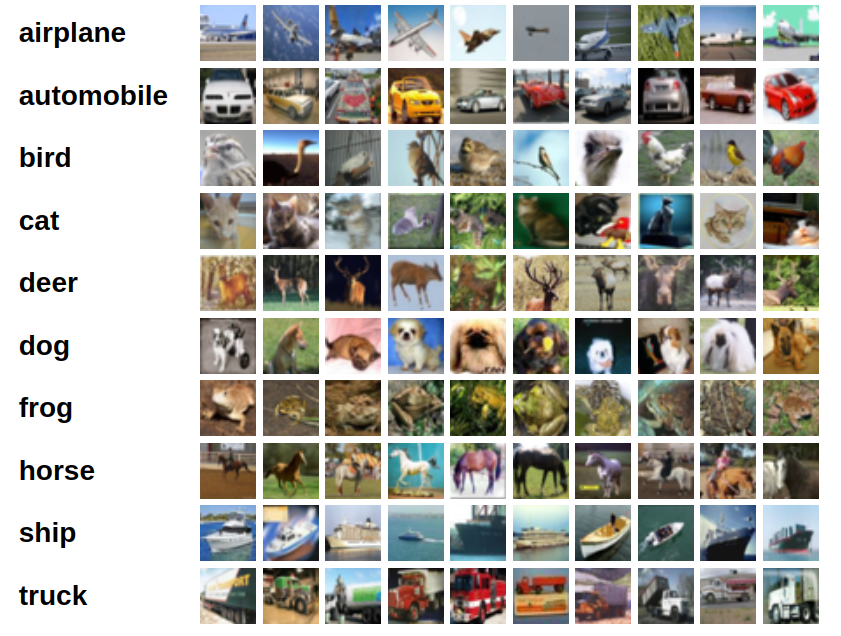
\includegraphics[width=10cm]{images_pfe/cifar-10-classes.png}
  \caption{Les classes du jeu de données CIFAR-10.}
  \label{fig:cifar-10-classes}
\end{figure}
\FloatBarrier
\medskip

Le dataset est divisé en deux ensemble: un ensemble d'entraînement et un ensemble de test. L'ensemble d'entraînement est composé de 50 000 images, tandis que l'ensemble de test est composé de 10 000 images. Dans ce dataset, les images sont de résolution relativement basse et présentent une variabilité dans les poses, l'éclairage, les arrière-plans et les détails, ce qui rend le dataset proche des défis du monde réel. Il est souvent utilisé pour l'entraînement, l'évaluation et la comparaison des performances des algorithmes de classification d'images et des réseaux de neurones convolutionnels (CNN), et il permet de reconnaître leur capacité à généraliser à partir d'un ensemble d'apprentissage limité [\cite{krizhevsky2009learning}].

\subsection{VGG-19}
VGG-19 \footnote{acronyme de "Visual Geometry Group" (famille des modèles développés par l'Université d'Oxford)} est un réseau de neurones convolutif (CNN) très profond qui possède plus de 19,6 milliards de FLOPs et est utilisé fréquemment dans le domaine de la vision par ordinateur. Il est composé de 19 couches, comprenant 16 couches de convolution et 3 couches entièrement connectées, et les images en entrée sont généralement de taille 224x224 pixels. Le réseau commence par des couches de convolutions successives, qui sont suivies de couches de pooling (de type max pooling). Ces dernières permettent de réduire la dimension spatiale de la sortie en ne conservant que les informations les plus importantes [\cite{simonyan2014very}].

Chaque couche de convolution est composée de plusieurs filtres (ou noyaux) 3x3 et un padding (stride) de 1 pour préserver les dimensions. Les filtres possèdent 64, 128, 256, 512 et 512 canaux respectivement. Le nombre de canaux augmente à mesure que l'on progresse dans le réseau. tandis que dans les couches de pooling, on a des fenêtres de 2x2 et un décalage de 2 pour réduire la résolution spatiale [\cite{simonyan2014very}]. 

Une fois que les données sont réduites en termes de dimensions spatiales, elles sont passées à travers plusieurs couches entièrement connectées afin d'effectuer la classification, en associant les caractéristiques apprises aux classes d'objets. La dernière couche de sortie possède le même nombre de neurones que de classes dans le jeu de données. Elle utilise une fonction d'activation softmax pour obtenir des probabilités normalisées pour chaque classe. Dans les couches de convolution, les fonctions d'activation utilisées sont des fonctions ReLU (Rectified Linear Unit) [\cite{simonyan2014very}].

\begin{table}[h!]
\begin{tabularx}{1.0\textwidth} { 
  | >{\centering\arraybackslash}X
  | >{\centering\arraybackslash}X 
  | >{\centering\arraybackslash}X
  | >{\centering\arraybackslash}X
  | >{\centering\arraybackslash}X
  | >{\centering\arraybackslash}X | }
 \hline
 \multicolumn{6}{|c|}{ConvNet Confguration} \\
 \hline
A & A-LRN & B & C & D & E \\
\hline
11 weight layers & 11 weight layers & 13 weight layers & 16 weight layers & 16 weight layers & 19 weight layers \\
\hline
\multicolumn{6}{|c|}{input(224 x 224 RGB image)} \\
\hline
conv 3-64 & conv 3-64 \textbf{LRN} & conv 3-64 \textbf{conv 3-64} & conv 3-64 conv 3-64 & conv 3-64 conv 3-64 & conv 3-64 conv 3-64 \\
\hline
\multicolumn{6}{|c|}{maxpool} \\
\hline
conv 3-128 & conv 3-128 & conv 3-128 \textbf{conv 3-128} & conv 3-128 conv 3-128 & conv 3-128 conv 3-128 & conv 3-128 conv 3-128 \\
\hline
\multicolumn{6}{|c|}{maxpool} \\
\hline
conv 3-256 conv 3-256 & conv 3-256 conv 3-256 & conv 3-256 conv 3-256 & conv 3-256 conv 3-256 \textbf{conv 1-256} & conv 3-256 conv 3-256 \textbf{conv 3-256} & conv 3-256 conv 3-256 conv 3-256 \textbf{conv 3-256} \\
\hline
\multicolumn{6}{|c|}{maxpool} \\
\hline
conv 3-512 conv 3-512 & conv 3-512 conv 3-512 & conv 3-512 conv 3-512 & conv 3-512 conv 3-512 \textbf{conv 1-512} & conv 3-512 conv 3-512 \textbf{conv 3-512} & conv 3-512 conv 3-512 conv 3-512 \textbf{conv 3-512} \\
\hline
\multicolumn{6}{|c|}{maxpool} \\
\hline
conv 3-512 conv 3-512 & conv 3-512 conv 3-512 & conv 3-512 conv 3-512 & conv 3-512 conv 3-512 \textbf{conv 1-512} & conv 3-512 conv 3-512 \textbf{conv 3-512} & conv 3-512 conv 3-512 conv 3-512 \textbf{conv 3-512} \\
\hline
\multicolumn{6}{|c|}{maxpool} \\
\hline
\multicolumn{6}{|c|}{FC-4096} \\
\hline
\multicolumn{6}{|c|}{FC-4096} \\
\hline
\multicolumn{6}{|c|}{FC-1000} \\
\hline
\multicolumn{6}{|c|}{soft-max} \\
\hline
\end{tabularx}
\caption{Les configurations des réseaux VGG (illustrées dans des colonnes selon leurs profondeurs). La colonne E représente la configuration du modèle VGG-19 utilisé [\cite{simonyan2014very}].}
\label{table:vgg-configurations}
\end{table}

\subsection{ResNet-34}
ResNet-34 est un réseau de neurones résiduel profond, composé de 34 couches et possédant plus de 3,6 milliards de FLOPs. Ce type de réseau est caractérisé par l'utilisation de blocs résiduels, en introduisant des connexions résiduelles, également appelées connexions "skip", qui sautent une ou plusieurs couches. Cette caractéristique permet d'exploiter les avantages de la profondeur tout en évitant les problèmes de dégradation de performance qui surviennent lorsque les réseaux deviennent plus profonds [\cite{He_2016_CVPR}].

Le bloc résiduel de base dans ResNet-34 comprend deux couches de convolution 3x3 accompagnées de fonctions d'activation ReLU, et intègre une connexion résiduelle qui agit comme un raccourci autour des couches de convolution, en ajoutant la sortie de la première couche de convolution à la sortie de la deuxième couche. 

\begin{figure}[hbt!]
  \centering
  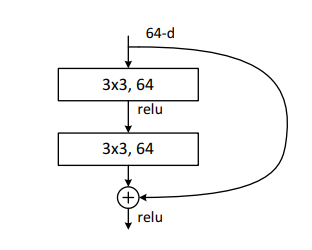
\includegraphics[width=10cm]{images_pfe/residual-bloc.png}
  \caption{Un bloc résiduel de base comme sur la figure \ref{fig:architectures} pour ResNet-34 [\cite{He_2016_CVPR}].}
  \label{fig:residual-bloc}
\end{figure}
\FloatBarrier
\medskip

La fin du réseau ResNet-34 comprend une couche de classification entièrement connectée avec autant de neurones que de classes dans le jeu de données. Une fonction d'activation softmax est généralement utilisée pour obtenir les probabilités de classe normalisées.

\begin{figure}[hbt!]
  \centering
  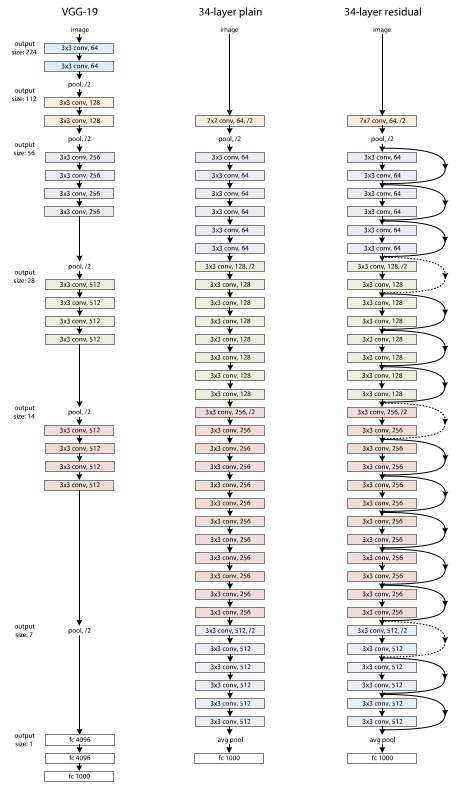
\includegraphics[width=13.5cm]{images_pfe/vgg-19-and-resnet-34.png}
  \caption{Les architectures des modèles utilisés. A gauche: le modèle VGG-19. Au milieu: un réseau simple de 34 couches. À droite: le modèle ResNet-34 [\cite{He_2016_CVPR}].}
  \label{fig:architectures}
\end{figure}
\FloatBarrier
\medskip

\section{Technologies utilisées}
\subsection{Python}

\begin{figure}[hbt!]
  \centering
  
\includegraphics[width=4cm]{images_pfe/python.png}
  \caption{Python.}
  \label{fig:python}
\end{figure}
\FloatBarrier
\medskip

Python joue un rôle important dans le domaine de l'intelligence artificielle (IA) grâce à sa polyvalence, sa simplicité et sa richesse en bibliothèques spécialisées. En tant que langage de programmation, Python est devenu le premier choix  pour de nombreux chercheurs, ingénieurs et développeurs travaillant dans le domaine de l'IA. D'une part, Python est connu pour sa syntaxe claire et lisible, ce qui  permet aux nouveaux arrivants dans le domaine de l'IA de se familiariser rapidement avec les concepts de base. D'autre part, Python offre plusieurs bibliothèques et frameworks spécialisés dans l'IA, tels que TensorFlow, Keras, PyTorch et Scikit-learn. Ces bibliothèques sont souvent utilisées pour le développement de réseaux de neurones, d'algorithmes d'apprentissage automatique et d'autres techniques d'IA. Finalement, Python est un langage polyvalent qui permet aux développeurs de créer et tester différentes approches rapidement.

\section{Bibliothèque utilisées}
Python offre une riche collection de bibliothèques spécialisées dans plusieurs domaines, en particulier l'IA. Ces bibliothèques offrent des outils et des frameworks puissants pour développer des modèles d'apprentissage automatique, des réseaux de neurones, et bien plus encore. Dans cette section, nous allons explorer les bibliothèques que nous avons utilisé pour implémenter et tester notre méthode.
\subsection{NumPy}

\begin{figure}[hbt!]
  \centering
  
\includegraphics[width=4cm]{images_pfe/numpy.png}
  \caption{NumPy.}
  \label{fig:numpy}
\end{figure}
\FloatBarrier
\medskip

NumPy \footnote{acronyme de "Numerical Python"} est une bibliothèque open source qui offre de nombreuses fonctionnalités pour le calcul numérique en Python. Elle offre un support puissant pour la manipulation de tableaux multidimensionnels, ainsi que pour l'exécution de calculs mathématiques complexes sur ces tableaux. Ces tableaux multidimensionnels permettent de stocker et de manipuler efficacement des données numériques sous forme de matrices et de vecteurs. Elle fournit également des fonctions mathématiques de base, des opérations d'algèbre linéaire, des opérations sur les tableaux, des fonctions statistiques et bien plus encore. Elle est largement utilisé en IA pour le traitement et la manipulation de données, la préparation de jeux de données, ainsi que pour la mise en œuvre d'algorithmes d'apprentissage automatique et de réseaux de neurones. La performance élevée de NumPy en calcul numérique en fait un bon choix pour les tâches intensives en termes de calcul.


\subsection{Matplotlib}
\begin{figure}[hbt!]
  \centering
  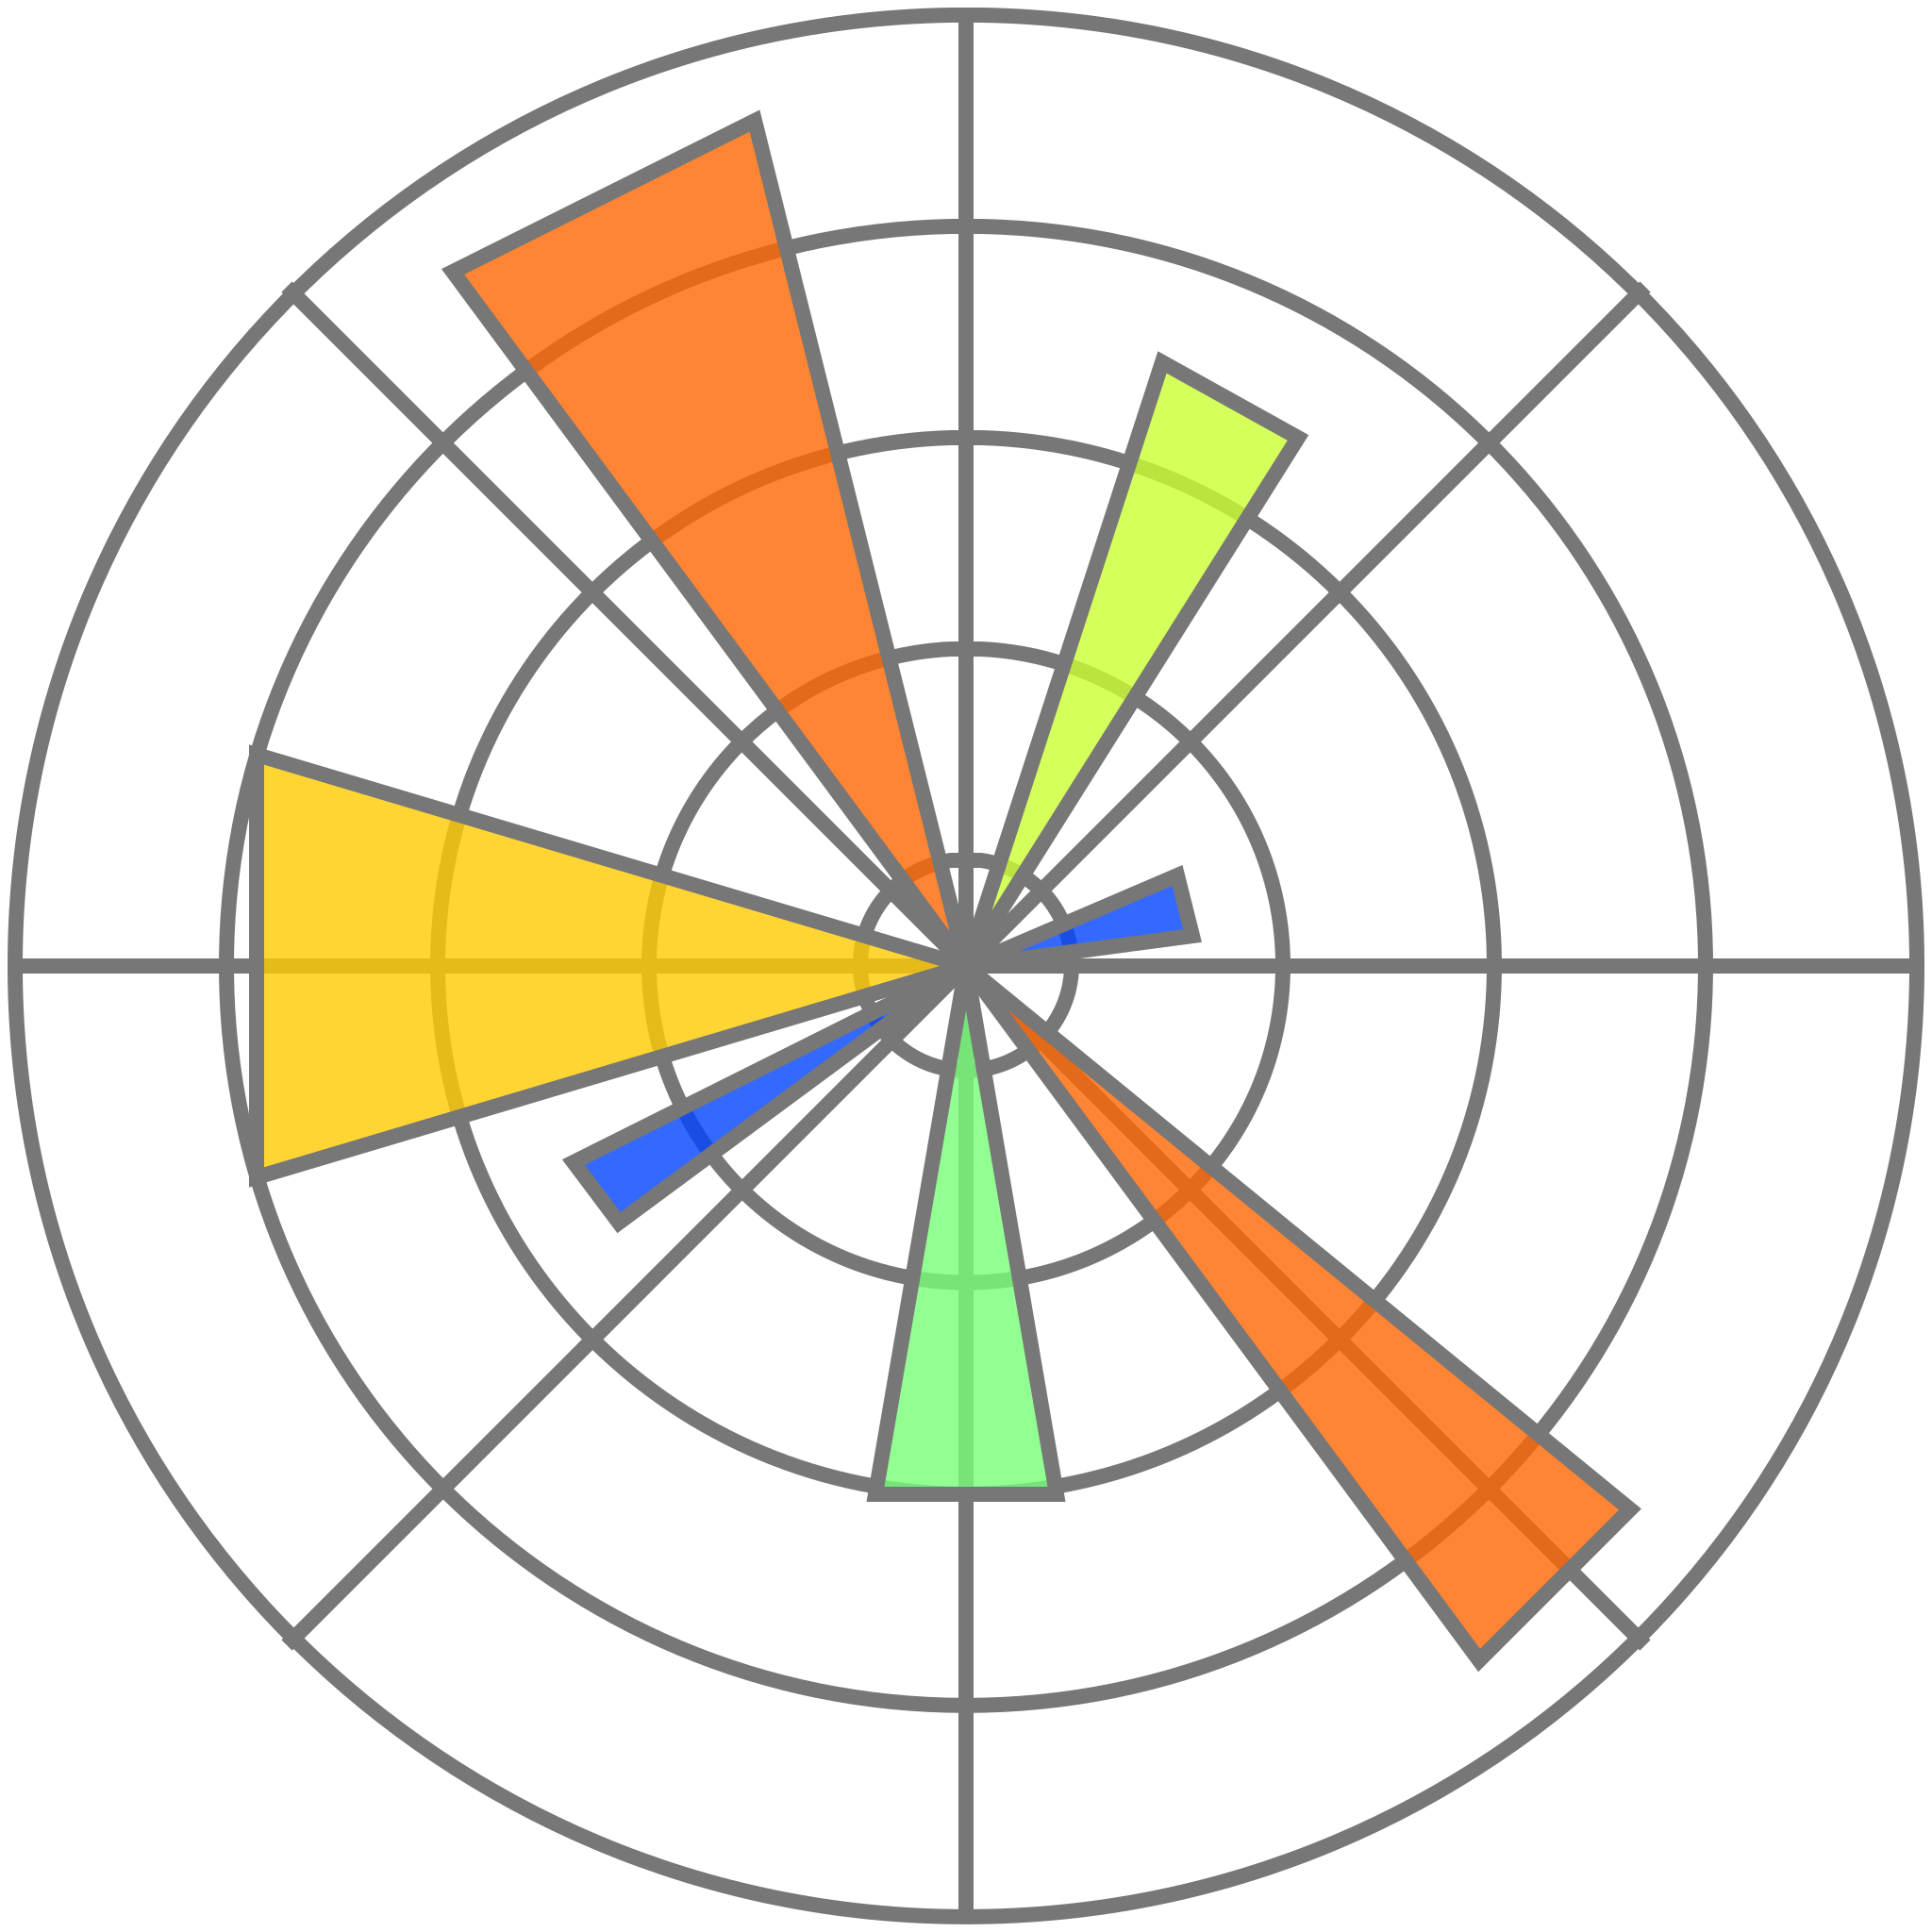
\includegraphics[width=4.5cm]{images_pfe/matplotlib.png}
  \caption{Matplotlib.}
  \label{fig:matplotlib}
\end{figure}
\FloatBarrier
\medskip

Matplotlib est une bibliothèque de visualisation en Python qui aide à créer des graphiques et des visualisations de données de manière interactive et statique. Cette bibliothèque offre un large éventail d'outils pour générer des graphiques de haute qualité à partir de données numériques. Son objectif est de permettre aux utilisateurs de représenter visuellement des données complexes de manière claire et compréhensible. Pour cela, elle propose une grande variété de types de graphiques, tels que les graphiques linéaires, les graphiques en barres, les graphiques à secteurs, les graphiques de dispersion, les graphiques 3D, etc. Elle permet également de personnaliser presque tous les aspects des graphiques, y compris les étiquettes, les couleurs, les styles de ligne, les titres, les axes et les légendes. L'utilisation de Matplotlib est essentielle dans l'analyse de données, la science des données et la recherche en général. En intelligence artificielle et en apprentissage automatique, Matplotlib est souvent employé pour visualiser les performances des modèles, les distributions de données, les tendances, les caractéristiques importantes, les matrices de confusion, les courbes d'apprentissage, etc.

\subsection{Pytorch}

\begin{figure}[hbt!]
  \centering
  
\includegraphics[width=4cm]{images_pfe/pytorch.png}
  \caption{Pytorch.}
  \label{fig:pytorch}
\end{figure}
\FloatBarrier
\medskip

PyTorch est une bibliothèque open-source d'apprentissage automatique et d'intelligence artificielle en Python, développée principalement par Facebook's AI Research lab (FAIR). Elle repose sur un concept fondamental appelé "tenseur", qui est une structure de données multidimensionnelle similaire aux tableaux NumPy et elle est conçue pour faciliter le développement et la mise en œuvre de modèles de réseaux de neurones profonds. PyTorch est surtout distinguée par sa prise en charge des calculs automatiques de gradients, ce qui signifie qu'il est possible de définir des opérations mathématiques sur les tenseurs et que PyTorch peut automatiquement calculer les gradients de ces opérations qui sont nécessaires pour ajuster les poids dans les réseaux de neurones et ainsi minimiser une fonction de perte. Elle est utilisé pour la conception des modèles de réseaux de neurones profonds, y compris les réseaux de neurones convolutionnels (CNN), les réseaux de neurones récurrents (RNN), les transformeurs, etc.

\subsection{Torchvision}

\begin{figure}[hbt!]
  \centering
  
\includegraphics[width=4cm]{images_pfe/torchvision.png}
  \caption{Torchvision.}
  \label{fig:torchvision}
\end{figure}
\FloatBarrier
\medskip

Torchvision est une bibliothèque qui fait partie de PyTorch. Elle est spécifiquement conçue pour faciliter le chargement et la transformation de jeux de données d'images couramment utilisés dans le domaine de l'apprentissage automatique et de la vision par ordinateur. Elle offre des outils pour prétraiter les données d'image, créer des ensembles de données, appliquer des transformations aux images et charger des ensembles de données préexistants. Elle propose des classes pour charger facilement des ensembles de données standard tels que MNIST, CIFAR-10, ImageNet, etc. Elle permet également d'appliquer diverses transformations aux images, telles que le redimensionnement, le recadrage, la normalisation, les rotations, les miroirs, etc. qui sont utiles pour augmenter la variabilité des données.

\subsection{NNI}

\begin{figure}[hbt!]
  \centering
  
\includegraphics[width=6cm]{images_pfe/nni.png}
  \caption{NNI (Neural Network Intelligence).}
  \label{fig:nni}
\end{figure}
\FloatBarrier
\medskip

NNI (Neural Network Intelligence) est une bibliothèque open-source développée par Microsoft Research. Elle fournit un ensemble d'outils et de bibliothèques pour faciliter l'exploration et l'optimisation des espaces d'hyperparamètres, ainsi que pour la recherche automatique d'architectures de modèles. Elle permet aux utilisateurs de définir un espace de recherche pour les hyperparamètres, tels que les taux d'apprentissage, les tailles de lot, les architectures de couches, etc. NNI exécute ensuite des expériences en utilisant différentes configurations d'hyperparamètres et rapporte les résultats, y compris les performances du modèle. Elle est très utile dans le domaine de l'apprentissage automatique, car elle simplifie et automatise le processus d'ajustement des hyperparamètres et d'exploration des architectures, ce qui peut considérablement accélérer le développement de modèles performants.

\section{Outils utilisés}

\subsection{Google Colab}

\begin{figure}[hbt!]
  \centering
  
\includegraphics[width=7cm]{images_pfe/colab.png}
  \caption{Google Colab.}
  \label{fig:colab}
\end{figure}
\FloatBarrier
\medskip

Google Colab (abrégé de Colaboratory) est une plateforme de notebooks interactifs basée sur le cloud, développée par Google. Elle permet aux utilisateurs d'écrire, d'exécuter et de partager du code Python de manière collaborative, sans nécessiter de configuration ou d'installation. Elle propose des notebooks interactifs qui permettent d'insérer des cellules de code exécutable et des cellules de texte et chaque notebook Colab s'exécute dans un environnement virtuel où les utilisateurs peuvent accéder à la puissance de calcul des processeurs graphiques (GPU) et des unités de traitement tensoriel (TPU) pour accélérer l'entraînement de modèles d'apprentissage automatique. Elle propose également de nombreuses bibliothèques préinstallées, mais les utilisateurs peuvent également installer et utiliser des bibliothèques tierces via des commandes simples.

\subsection{Google Drive}

\begin{figure}[hbt!]
  \centering
  
\includegraphics[width=6cm]{images_pfe/drive.png}
  \caption{Google Drive.}
  \label{fig:drive}
\end{figure}
\FloatBarrier
\medskip

Google Drive est un service de stockage en ligne développé par Google pour stocker, synchroniser et partager des fichiers et des dossiers sur le cloud. Il offre une variété de fonctionnalités telles que le stockage en ligne, la synchronisation multi-appareils, le partage de fichiers, la collaboration en temps réel, etc. De plus, il peut être utilisé avec Google Colab.

\section{Tests et résultats}
Cette dernière section présente une analyse des résultats obtenus après avoir tester notre méthode d'élagage. Nous effectuons nos expérimentations sur CIFAR-10 avec deux réseaux profonds classiques: VGG-19 et ResNet-34. Les résultats obtenus sont examinés et comparés avec les résultats des autres méthodes d'élagage, permettant ainsi de dégager des conclusions quant à la performance et l'efficacité de notre méthode. Cette section donc vise à présenter de manière claire et précise les découvertes issues de ces tests.

Le processus d'exécution des tests est décrit comme suit:
\begin{enumerate}
    \item Entraînement du modèle jusqu'à la convergence
    \item Élagage du modèle avec les pourcentages d'élagage fournis par l'agent DDPG
    \item Réglage fin du modèle
    \item Mesure de la précision, la taille, le nombre de paramètres, etc. du modèle élagué
    \item Comparaison du modèle élagué avec le modèle original
\end{enumerate}

On élague les canaux dont les poids ont la plus petite valeur absolue. Le pourcentage d'élagage maximum $a_{max}$ est fixé pour les couches de convolution à 0,8 et pour la couche entièrement connectée à 0,98. Cette limite supérieure $a_{max}$ est utilisée uniquement pour accélérer la recherche. Nous pouvons simplement prendre $a_{max} = 1$ et nous aurons des résultats similaires. Le réseau d’acteurs $\mu$ comporte deux couches cachées, chacune comportant 300 neurones et la couche de sortie finale est une couche sigmoïde pour délimiter les actions dans la plage (0, 1). Le réseau critique \textit{Q} comportait également deux couches cachées, chacune comptant 300 unités. Nous entraînons le réseau avec 64 comme batch size. L'agent DDPG explore d’abord 100 épisodes avec un bruit constant $\sigma = 0.5$, puis exploite 300 épisodes avec un bruit $\sigma$ qui décroît de manière exponentielle.

Pour évaluer la performance de notre méthode, nous l'avons comparée avec les deux méthodes d'élagage citées dans la première partie du rapport: ABCPruner [\cite{lin2020channel}] et CCPrune [\cite{CHEN202135}]. Ces deux méthodes sont des méthodes automatique qui utilisent le même type d'élagage (élagage des canaux). ABCPruner est une méthode basée sur l'algorithme de colonie d'abeilles artificielles (ABC). Dans cette méthode, la recherche du réseau élagué optimal est formulée comme un problème d'optimisation et l'algorithme ABC est utilisé pour le résoudre de manière automatique afin de réduire les interférences humaines. CCPrune (Collaborative Channel Pruning) est une autre méthode qui utilise aussi l'élagage des canaux. Cette méthode introduit d’abord la régularisation sur les poids des couches de convolution et les facteurs d’échelle de la couche BN (Batch Normalization) respectivement, puis elle combine les poids de la couche de convolution et le facteur d’échelle de la couche BN pour évaluer l’importance du canal.

\clearpage

\subsection{VGG-19}
Le tableau suivant représente les résultats après l'application de notre méthode sur VGG-19 avec une comparaison aux deux autres méthodes d'élagage: ABCPruner et CCPrune.

\begin{table}[h!]
\begin{tabular}{|p{3.25cm}|p{3cm}|p{2.25cm}|p{3cm}|p{2.25cm}|}
\hline
Méthode & Précision (\%) & FLOPs (\%) & Paramètres (\%) & Taille (MB) \\
\hline
Modèle original & 93.71 & - & - & 548 \\
\hline
ABCPruner & 93.08 & 73.68 & 88.68 & 62.6 \\
\hline
CCPrune & \textbf{93.78} & 48.92 & 86.82 & 77.2 \\
\hline
Notre méthode & 90.6 & 91.6 & 90.2 & \textbf{52.7} \\
\hline
\end{tabular}
\caption{Résultats d'élagage de VGG-19 sur CIFAR-10. La deuxième colonne indique la précision du modèle. Les troisième et quatrième colonnes indiquent le taux d'élagage des FLOPs et le taux d'élagage des paramètres. La dernière colonne indique la taille du modèle.}
\label{table:vgg-pruning-results}
\end{table}

Les résultats dans le tableau \ref{table:vgg-pruning-results} montrent que les techniques ABCPruner et CCPrune atteignent toujours une précision très proche du réseau original qui est aussi meilleure que celle de notre méthode. Cependant, notre méthode dépasse ces techniques quand nous parlons de la taille du modèle. Nous remarquons qu'avec notre méthode, nous pouvons d'avoir une grande réduction dans la taille du modèle (la taille est 10 fois moins que le modèle original) et dans le nombre de FLOPs et paramètres à cause des pourcentages d'élagage élevés. Cette réduction du nombre de FLOPs signifie que notre méthode effectue moins de calculs que les deux autres méthodes. Nous pouvons donc avoir le meilleur temps d'inférence avec notre méthode. Nous pouvons aussi remarquer que l'utilisation de l'élagage structuré engendre une petite dégradation de la précision des modèles élagués par rapport au modèle original. Cette dégradation est causée par la suppression de canaux entiers, ce qui peut causer une suppression de certains paramètres importants qui peuvent se trouver dans l'un des canaux éliminées.

La figure \ref{fig:vgg-channels} montre les statistiques des canaux restants dans les couche de convolution dans le modèle VGG-19. Sur cette figure, Nous pouvons clairement comprendre la structure du réseau après l'élagage.

Dans VGG-19, 90\% des poids sont dans les couches entièrement connectées. Dans notre méthode, nous avons utilisé l’élagage de canaux entiers en couches de convolution et cela a un effet secondaire intéressant en réduisant également la mémoire. Comme observé dans \cite{molchanov2016pruning}, plus la couche est profonde, plus elle sera élaguée. Cela signifie que la dernière couche de convolution sera beaucoup élaguée et que de nombreux neurones de la couche entièrement connectée qui la suit seront également supprimés.

\begin{figure}[hbt!]
  \centering
  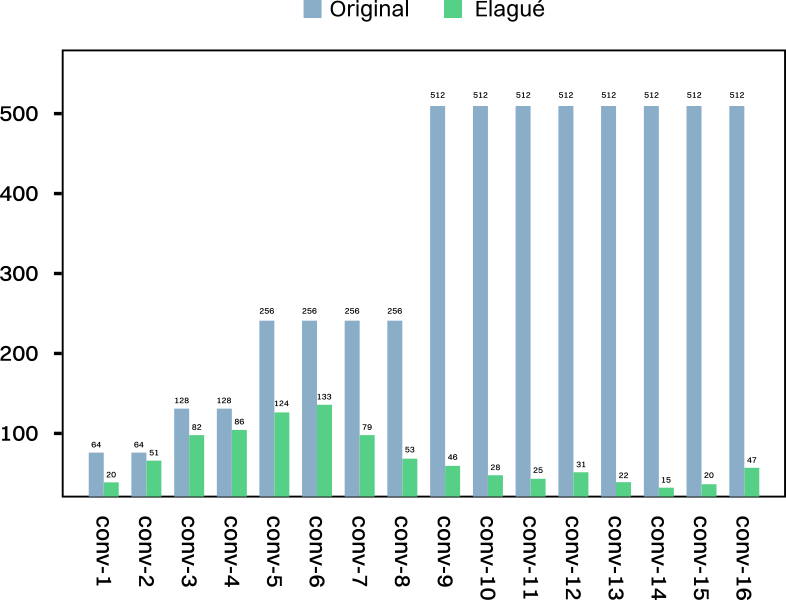
\includegraphics[width=14cm]{images_pfe/vgg-channels.png}
  \caption{Statistiques des canaux restants dans les couches de convolution de VGG-19.}
  \label{fig:vgg-channels}
\end{figure}
\FloatBarrier
\medskip

\subsection{ResNet-34}
Le tableau suivant représente les résultats après l'application de notre méthode sur ResNet-34 et une comparaison avec les deux autres méthodes d'élagage utilisées: ABCPruner et CCPrune.

\begin{table}[h!]
\begin{tabular}{|p{3.25cm}|p{3cm}|p{2.25cm}|p{3cm}|p{2.25cm}|}
\hline
Méthode & Précision (\%) & FLOPs (\%) & Paramètres (\%) & Taille (MB) \\
\hline
Modèle original & 91.45 & - & - & 81.4 \\
\hline
ABCPruner & 89.69 & 58.97 & 51.76 & 39.2 \\
\hline
CCPrune & \textbf{90.76} & 57.55 & 34.78 & 53.0 \\
\hline
Notre méthode & 86.21 & 58.09 & 67.63 & \textbf{26.5} \\
\hline
\end{tabular}
\caption{Résultats d'élagage de ResNet-34 sur CIFAR-10. La deuxième colonne indique la précision du modèle. Les troisième et quatrième colonnes indiquent le taux d'élagage des FLOPs et le taux d'élagage des paramètres. La dernière colonne indique la taille du modèle.}
\label{table:resnet-pruning-results}
\end{table}

Les résultats dans le tableau \ref{table:resnet-pruning-results} sont les même que ceux du modèle
VGG-19. Ils montrent toujours que la précision dans les techniques ABCPruner et CCPrune dépasse la précision dans notre méthode. Cependant, notre méthode dépasse ces deux techniques dans la compression de la taille du modèle et dans le nombre de FLOPs, ce qui nous donnera un meilleur temps d'inférence. Nous remarquons aussi que la taille du modèle élagué avec notre méthode est presque 3 fois moins que le modèle original, ainsi que le nombre de FLOPs et paramètres (les résultats sont résumés dans la figure \ref{fig:resnet-pruning}). Nous avons aussi vu que l'élagage structuré réduit légèrement la précision des modèles élagués par rapport au modèle original et la cause de cette réduction est la même cause mentionnée dans l’interprétation de l’élagage structuré pour le modèle VGG-19.

\begin{figure}[hbt!]
  \centering
  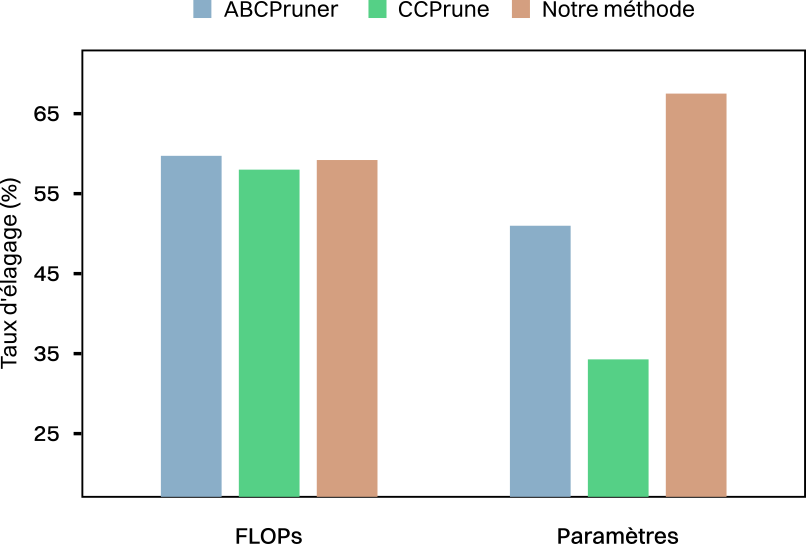
\includegraphics[width=14cm]{images_pfe/resnet-pruning.png}
  \caption{Comparaison entre les taux d'élagage des FLOPs et des paramètres des trois méthodes d'élagage pour le réseau ResNet-34.}
  \label{fig:resnet-pruning}
\end{figure}
\FloatBarrier
\medskip

\section{Conclusion}
En conclusion de ce chapitre dédié aux tests et résultats, l'analyse des résultats d'expérimentations menées sur les modèles VGG-19 et ResNet-34 prouvent l'efficacité de notre méthode d'élagage automatique. Nous avons trouvé que notre méthode permet de réduire significativement la taille des modèles et le nombre de FLOPs, en surpassant les deux méthodes utilisées pour la comparaison (ABCPruner et CCPrune). Ces réductions nous permettent d'avoir de très petits modèles qui sont également très performants et faciles à déployer sur des appareils limités en termes de ressources de calcul et de stockage. Cependant, il est important de souligner que le processus d'élagage n'est pas sans compromis. Les avantages en termes de taille sont parfois accompagnés d'une petite dégradation de la précision qui nécessite de faire un réglage fin après l'élagage afin de restaurer partiellement les performances du modèle initial. De plus, le taux d'élagage optimal peut varier en fonction du même jeu de données et des spécificités de la tâche.

On a également présentée au début du chapitre les modèles utilises pour tester la méthode (VGG-19 et ResNet-34) et le jeu de données utilisé (CIFAR-10) pour l'entraînement de ces modèles, ainsi que les différents technologies et outils utilisés pour la conception de notre méthode. Nous avons utilisé le langage de programmation Python avec plusieurs bibliothèques telles que NumPy, Matplotlib, Pytorch, etc. Ces bibliothèques offrent des outils puissants pour développer et entraîner les différents types de réseaux de neurones.

Enfin, ce chapitre constitue une étape essentielle de ce rapport en fournissant des résultats d'implémentation des concepts et des théories énoncés dans le chapitre précédent. Les résultats obtenus offrent des orientations pratiques pour les applications et les améliorations futures de cette méthode pour élaguer des réseaux de neurones profonds. En considérant ces résultats, la rapport se tourne vers la section finale, où les conclusions et perspectives globales sont tirées.
